% =============================================================================
% math-venn-two-set.tex — Two-set Venn diagram with labelled regions
%
% Shows: sets A and B inside a universe rectangle, with the intersection
% shaded and all four regions labelled.
% Compiles standalone via: xelatex math-venn-two-set.tex
%
% Use for: discrete mathematics (set algebra, inclusion-exclusion), probability
% (events, conditional probability), logic (predicate overlap).
%
% For THREE sets, place circle centres on an equilateral triangle of side 1.5r
% and expect seven regions — label them outside with leader lines rather than
% cramming text into the small central region.
% =============================================================================

\documentclass[border=5pt]{standalone}
\usepackage{tikz}
\usetikzlibrary{arrows.meta, positioning}

\definecolor{setA}{HTML}{012169}
\definecolor{setB}{HTML}{B9975B}
\definecolor{inter}{HTML}{15803D}
\definecolor{muted}{HTML}{525252}

\tikzset{
  setcircle/.style={thick, draw=#1, fill=#1, fill opacity=0.13, draw opacity=1},
  universe/.style={draw=muted, thick, rounded corners=2pt},
  reglbl/.style={font=\small},
  setlbl/.style={font=\small\bfseries}
}

% -----------------------------------------------------------------------------
% Diagram: A and B overlapping inside universe U.
% Coordinates: (x, y)
%   Circle A centre (-0.85, 0), radius 1.7
%   Circle B centre ( 0.85, 0), radius 1.7
%   Overlap spans x in [-0.85, 0.85]; the lens is 1.7cm wide at its waist, so
%   the "A ∩ B" label fits at the origin without touching either arc.
%   Universe rectangle from (-3.4, -2.2) to (3.4, 2.2) — 0.85cm clear of the
%   circles' outer edges (A's left edge is at -2.55) (P7c).
% Region labels sit at the CENTROID of each region, not on an arc:
%   A only at (-1.75, 0) ; B only at (1.75, 0) ; A ∩ B at (0, 0)
%   Neither-set label in the top-left corner of the universe, clear of both.
% Set names sit ABOVE their circles, outside the arcs.
% -----------------------------------------------------------------------------

\begin{document}
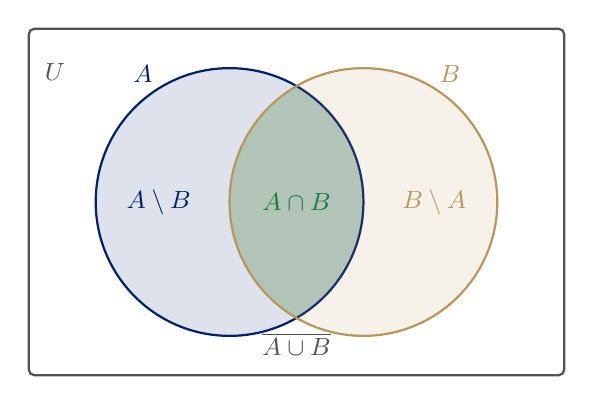
\begin{tikzpicture}

  % ---- Universe ------------------------------------------------------------
  \draw[universe] (-3.4, -2.2) rectangle (3.4, 2.2);
  \node[reglbl, text=muted, above right] at (-3.32, 1.42) {$U$};

  % ---- Shaded intersection (drawn first, under the outlines) --------------
  \begin{scope}
    \clip (-0.85, 0) circle (1.7);
    \fill[inter, fill opacity=0.22] (0.85, 0) circle (1.7);
  \end{scope}

  % ---- The two sets --------------------------------------------------------
  \draw[setcircle=setA] (-0.85, 0) circle (1.7);
  \draw[setcircle=setB] ( 0.85, 0) circle (1.7);

  % ---- Set names, above and outside the arcs ------------------------------
  \node[setlbl, text=setA] at (-1.95,  1.62) {$A$};
  \node[setlbl, text=setB] at ( 1.95,  1.62) {$B$};

  % ---- Region labels at region centroids ----------------------------------
  \node[reglbl, text=setA]  at (-1.75, 0) {$A \setminus B$};
  \node[reglbl, text=inter] at ( 0.00, 0) {$A \cap B$};
  \node[reglbl, text=setB]  at ( 1.75, 0) {$B \setminus A$};
  \node[reglbl, text=muted] at ( 0.00, -1.80) {$\overline{A \cup B}$};

\end{tikzpicture}
\end{document}
